\documentclass[12pt, letterpaper]{article}
\usepackage[utf8]{inputenc}
\usepackage{graphicx}

\graphicspath{{./}}

\title{General refactor of "carstatus.cpp"}
\date{2019 November 15}
%\authors{Thomas De Min}

\begin{document}

\begin{titlepage}
\maketitle
\end{titlepage}

\begin{flushleft}

\section{Introduction}
	The SteeringWheel UI needs a lot of variables in order to works properly. In the past those variables were all putted toghether in one place, "Carstatus". This class was created to store them and to collect methods associated to them. To date "Carstatus" contains over 50 variables. At this point there is a lot of confusion and the code is difficult to be read.
\newline
\newline
\begin{figure}[h]
    \centering
    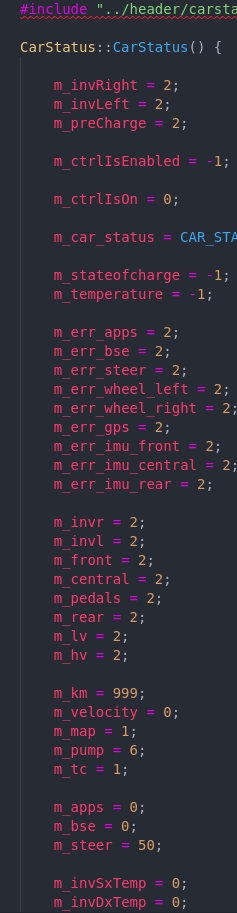
\includegraphics[scale=1.5]{code.png}
\end{figure}
\newline
\newline
	The ideal solution is to store variables and methods associated in different classes and use them from "Carstatus" using a "has a" for each class.\\
	---------------------------------------------INSERT CLASS DIAGRAM HERE-------------------------------------------------------

\section{Implementation issues}
	These changes will make code finally readable but some methods require to remain into "Carstatus". These methods are thoose that deal with sending changed data after emits.\\
	The only possible solution is to make some getters inside the new classes and call them from "Carstatus". Therefore there will still be functions in this class but there will be much less.\\
	Another side effect of this implementation is the needs to create a ".h" (and ".cpp") file for each new class. There will be more or less 10 new classes, that means 10 new header and source files.

\section{Refactor}
\subsection{Inverter}
\begin{verbatim}
int m_invRight;
int m_invLeft;
int m_preCharge;
int m_invSxTemp;
int m_invDxTemp;
\end{verbatim}
These 5 variables has been moved into a new Class called Inverters. Now Carstatus' functions use getter and setter of this class in order to maintain an object oriented paradigm. Variables' names are also changed to keep a certain standard.\\
So, the class now looks like this:
\begin{verbatim}
public:
    Inverters();
    void setLeftInverter(int);
    void setRightInverter(int);
    void setPreCharge(int);
    void setLeftInverterTemperature(int, int);
    void setRightInverterTemperature(int, int);
    int getLeftInverter() const;
    int getRightInverter() const;
    int getPreCharge() const;
    int getLeftInverterTemperature() const;
    int getRightInverterTemperature() const;
private:
    int invLeft;
    int invRight;
    int preCharge;
    int invLeftTemp;
    int invRightTemp;
\end{verbatim}

\subsection{Control}
\begin{verbatim}
int m_ctrlIsEnabled;
int m_ctrlIsOn;
int m_car_status;
\end{verbatim}
These 3 has been moved into Control class with respective getters and setters
\begin{verbatim}
public:
    Control();
    void setCtrlIsEnabled(bool);
    void setCtrlIsOn(bool);
    bool setCarStatus(int);
    bool getCtrlIsEnabled() const;
    bool getCtrlIsOn() const;
    int getCarStatus() const;
private:
    bool ctrlIsEnabled;
    bool ctrlIsOn;
    int carStatus;
\end{verbatim}
As you could notice \begin{verbatim}ctrlIsEnabled\end{verbatim} and \begin{verbatim}ctrlIsOn\end{verbatim} now are boolean. This decision was taken because these variables rappresent boolean values and two integers were a waste of resources.

\end{flushleft}

\subsection{Race}
\begin{verbatim}
int m_speed;
int m_velocity;
int m_km;
\end{verbatim}
These 3 have been moved into the new Race class with respective getters and setters.\newline
The new Race class looks like:
\begin{verbatim}
public:
    Race();
    void setSpeed(int, int);
    void setVelocity(int);
    void setKm(int, int);
    int getSpeed() const;
    int getVelocity() const;
    int getKm() const;
private:
    int speed;
    int velocity;
    int km;
\end{verbatim}
In order to maintain the new standard the formulas to calcolate speed and km has been inserted into setSpeed and setKm functions, this could not be done for setVelocity function because in carStatus.cpp there are 2 different formulas to calcolate the velocity, so it is easier to maintain that formulas into carStatus.

\subsection{Warning}
\begin{verbatim}
int m_invr;
int m_invl;
int m_front;
int m_rear;
int m_lv;
int m_hv;
int m_central;
int m_pedals;
int m_warning;
\end{verbatim}
These old variables have been moved to Warning, the new class; as always the new class has all getters and setters required.\newline
The new Warning class looks like:
\begin{verbatim}
public:
    Warning();
    void setInvRight(int);
    void setInvLeft(int);
    void setFront(int);
    void setRear(int);
    void setLv(int);
    void setHv(int);
    void setCentral(int);
    void setPedals(int);
    void setWarning(int);
    int getInvRight() const;
    int getInvLeft() const;
    int getFront() const;
    int getRear() const;
    int getLv() const;
    int getHv() const;
    int getCentral() const;
    int getPedals() const;
    int getWarning() const;
private:
    int invRight;
    int invLeft;
    int front;
    int rear;
    int lv;
    int hv;
    int central;
    int pedals;
    int warning;
\end{verbatim}
The \textbf{Q\_PROPERTY} called warning in carStatus.h has been modified to getWarning (and valWarning for the variable name) in order to free the warning instace and to give it to the new Warning class instace. This means that all the references in qml to the older warning \textbf{Q\_PROPERTY} has been modified to getWarning or valWarning. The file in question is StatusLED.qml. In this way it has been possible to maintain our new standard.\newline
Schematically:
\begin{itemize}
    \item Older \textbf{Q\_PROPERTY} in carStatus:
    \begin{verbatim}
    Q_PROPERTY(int warning READ warning NOTIFY warningChanged);
    \end{verbatim}
    \item New \textbf{Q\_PROPERTY} in carStatus:
    \begin{verbatim}
    Q_PROPERTY(int varWarning READ getWarning NOTIFY warningChanged);
    \end{verbatim}
    \item Older \textbf{StatusLED.qml}:
    \begin{verbatim}
    property var warning : CarStatus.warning;
    ...
    warningVal = CarStatus.warning;
    \end{verbatim}
    \item New \textbf{StatusLED.qml}:
    \begin{verbatim}
    property var warning : CarStatus.getWarning;
    ...
    warningVal = CarStatus.varWarning;
    \end{verbatim}
\end{itemize}

\subsection{Manettini}
\begin{verbatim}
int m_map;
int m_tc;
int m_pump;
\end{verbatim}
These 3 variables belong to Steering Wheel's physical manettini which control respectively car's power delivery, traction control and cooling. These are now moved into Manettini class.
\begin{verbatim}
public:
    Manettini();
    void setMap(int);
    void setTc(int);
    void setPump(int);
    int getMap() const;
    int getTc() const;
    int getPump() const;
    void incMap(const int);
    void incPump(const int);
    void incTc(const int);
private:
    int map;
    int tc;
    int pump;
\end{verbatim}
As can be seen besides getters, setters and the class costructor, it has been also added 
\begin{verbatim}incMap incPump incTc.\end{verbatim}
Their task is to increment the value of each manettino by one, if this value exceeds a certain amount it runs a modulus in order to reset the variable.

\subsection{Errors}
\begin{verbatim}
int m_err_apps;
int m_err_bse;
int m_err_steer;
int m_err_wheel_left;
int m_err_wheel_right;
int m_err_gps;
int m_err_imu_front;
int m_err_imu_central;
int m_err_imu_rear;
int m_error;
\end{verbatim}
These 10 variables have been moved into Errors class. This also implements getters and setters.
\begin{verbatim}
public:
    Errors();
    void setErrApps(int);
    void setErrBse(int);
    void setErrSteer(int);
    void setErrLeftWheel(int);
    void setErrRightWheel(int);
    void setErrGps(int);
    void setErrFrontIMU(int);
    void setErrCentralIMU(int);
    void setErrRearIMU(int);
    void setError(int);
    void setAll(int, int, int, int, int, int, int, int, int);
    int getErrApps()const;
    int getErrBse()const;
    int getErrSteer()const;
    int getErrLeftWheel()const;
    int getErrRightWheel()const;
    int getErrGPS()const;
    int getErrFrontIMU()const;
    int getErrCentralIMU()const;
    int getErrRearIMU()const;
    int getError()const;
private:
    int err_apps;
    int err_bse;
    int err_steer;
    int err_wheel_left;
    int err_wheel_right;
    int err_gps;
    int err_imu_front;
    int err_imu_central;
    int err_imu_rear;
    int error;
\end{verbatim}
As can be seen, there also is a method named
\begin{verbatim}setAll.\end{verbatim}
This has been implement in order to simplify the readability of
\begin{verbatim}CarStatus::setErrStatus\end{verbatim}

\subsection{Sensors}
\begin{verbatim}
int m_brakeVal;
int m_throttleVal;
int m_apps;
int m_bse;
int m_steer;
int m_num_err_apps;
int m_num_err_bse;
int m_num_err_steer;
\end{verbatim}
These 8 variables have been moved into Sensors class:
\begin{verbatim}
public:
    Sensors();
    void setBrakeVal(int);
    void setThrottleVal(int);
    void setApps(int);
    void setBse(int);
    void setSteer(int);
    void setNumErrApps(int);
    void setNumErrBse(int);
    void setNumErrSteer(int);
    int getBrakeVal()const;
    int getThrottleVal()const;
    int getApps()const;
    int getBse()const;
    int getSteer()const;
    int getNumErrApps()const;
    int getNumErrBse()const;
    int getNumErrSteer()const;
private:
    int brakeVal;
    int throttleVal;
    int apps;
    int bse;
    int steer;
    int num_err_apps;
    int num_err_bse;
    int num_err_steer;
\end{verbatim}
Apart from getters and setters there were no changes.

\subsection{High Voltage}
\begin{verbatim}
    int m_hvTemp;
    int m_hvVolt;
\end{verbatim}
These 2 variables have been moved into Hv Class:
\begin{verbatim}
public:
    Hv();
    void setHvTemp(int, int);
    void setHvVolt(int, int , int);
    int getHvTemp() const;
    int getHvVolt() const;
private:
    int hvTemp;
    int hvVolt;
\end{verbatim}
Apart from getters and setters there were no changes.

\subsection{Low Voltage}
\begin{verbatim}
int m_lvTemp;
int m_lvVolt;
\end{verbatim}
These 2 have been moved into Lv Class:
\begin{verbatim}
public:
    Lv();
    void setLvTemp(int);
    void setLvVolt(int);
    int getLvTemp() const;
    int getLvVolt() const;
private:
    int lvTemp;
    int lvVolt;
\end{verbatim}
Apart from getters and setters there were no changes.

\subsection{Telemetry}
\begin{verbatim}
int telemetry[11];
bool sender;
int telemetryEnStatus;
int popup;
\end{verbatim}
These 4 hasn't been changed however they have been moved into a new Class called Telemetry:
\begin{verbatim}
public:
    Telemetry();
    void setTelemetry(int, int, int, int, int, int, int, int, int, int, int);
    void setSender();
    void setTelemetryStatus(int);
    void setPopupMessage(int);
    void setTelemetryIndex(int);
    int getTelemetry(int) const;
    bool getSender() const;
    int getTelemetryStatus() const;
    int getPopupMessage() const;
private:
    int telemetry[11];
    bool sender;
    int telemetryEnStatus;
    int popup;
\end{verbatim}

\end{document}